\documentclass[11pt]{article}
\usepackage[utf8]{inputenc}
\usepackage[T1]{fontenc}
\usepackage[francais]{babel}
\usepackage[francais]{layout}
\usepackage{hyperref}
\selectlanguage{french}

% NE PAS CHANGER !!
\ifx \public \undefined \def\public{etudiants} \fi
\usepackage[\public]{tps}
\usepackage{tikz}

% Numéro du TP
\newcommand{\numtd}{03}
% Titre du TP
\newcommand{\titretd}{Construction of a real computer}
\def\tup#1{\langle #1\rangle}
\begin{document}

\entete{\numtd}{\titretd}

\section{Introduction}

For this TP, you can find the UPDATED zip folder containing all the requisite files here: \url{https://www.amritasuresh.github.io/teaching/bootstrap.tar.gz}.

Continuing from last week's TP, we will finish our endeavour of building a small computer starting from (almost) scratch. 
%To do this we will build increasingly complicated logical units until we have a computer capable of running programs. For this lab, we will use a Hardware Simulator. Its role will be to check that your logical units (\textit{chips}) are well implemented. In addition, it will also help you with your debugging your chips.
%
%The language in which you will write your chips is a DSL (Domain Specific Language), i.e. a language specifically dedicated to the writing of your chips. In the next section, this language will be briefly introduced so that you can start writing your first chips. 
%
%Each chip consists of three files:
%\begin{itemize}
%\item \texttt{XXX.hdl} : this is the file that you will write the code of your chips in.
%\item \texttt{XXX.tst} : this is a pre-written file which contains tests to verify if your code is right.
%\item \texttt{XXX.cmp} : this is also pre-written with the output of the test file.
%\end{itemize}
%
%The last two files are used by the Hardware Simulator to check the correctness of your chips. So for the most part, you will only edit files with the extension \texttt{.hdl}.
%
%\subsection*{Using the Hardware Simulator}Once the Hardware Simulator is started, to check your chip you have to follow these steps:
%\begin{itemize}
%\item Click on the \textbf{load chip} button to load the \texttt{.hdl} file
%\item Click on the \textbf{load script} button to load the \texttt{.tst} file
%\item Finally, click the \textbf{run} button (blue double-arrow) to run the tests
%\end{itemize}
%
%To save time, you can select the \textbf{no animation} button in the \textbf{animation} menu.
%
%\subsection*{Plan}
%
%This TP is divided into \(4\) sections :
%\begin{enumerate}
%\item In Section~\ref{sec:base}, you have to implement the basic chipset : \texttt{And}, \texttt{Or}, ...
%\item In Section~\ref{sec:alu}, we are interested in the conception of an ALU (Arithmetic Logic Unit)
%\item In Section~\ref{sec:memory}, we are interested in non-sequential chips in order to create the memory (RAM) of our computer
%%\item In section~\ref{sec:computer},we will bring together the different CHIPS written in the previous sections to build the computer.
%\end{enumerate}
%
%\section{Hardware Language}
%
%\textit{Hardware Language} is a language that allows you to program chips. All the chips you are going to write respect the following format (example of the \texttt{AND} gate) :
%\begin{verbatim}
%/**
% * And gate:
% * out = 1 if (a == 1 and b == 1)
% *       0 otherwise
% */
%
%CHIP And {
%    IN a, b;
%    OUT out;
%
%    PARTS:
%    //TODO
%}
%\end{verbatim}
%
%Each chip begins with a comment summarizing the expected behavior of the chip. Then, the code of a chip is divided into three parts:
%\begin{itemize}
%\item \textit{IN} : this line gives names to the input pins. Here, the \texttt{AND} gate has two input pins named \texttt{a} and \texttt{b}
%\item \textit{OUT} :  this line gives names to the output pins. Here, the \texttt{AND} gate has a single output pin named \texttt{out}
%\item \textit{PART} : This part contains the program you are going to write to implement the chips. This part is made up of a sequence of \ texttt {instructions} (described below) separated by semicolons.
%\end{itemize}
%
%The format of an instruction is as follows:
%\begin{verbatim}
%XXX(ipin1=var1, ipin2=var2, ..., opin1=var3, opin2=var4, ...)
%\end{verbatim}
%
%The semantics of this instruction is that it calls the chip \texttt{XXX} :
%\begin{itemize}
%\item it connects to the input pin \texttt{ipin1} the pin \texttt{var1}, to the input pin \texttt{ipin2} the pin \texttt{var2}.
%\item \texttt{var3} is the new name of the output pin \texttt{opin1}, and \texttt{var4} is the new name of the output pin \texttt{opin2}
%\end{itemize}
%
%For the first two sections, it is expected that \texttt{var3} and \texttt{var4} are new names (new variables are created), while \texttt{var1} and \texttt{var2} are names that must already exist.
%
%For example, when you want to create a new chip and you want to use the \texttt{AND} chip, you can write the following instruction:
%\begin{verbatim}
%...
%AND(a=a1,b=a2, out=outand)
%\end{verbatim}
%
%assuming that the variables \texttt{a1} and \texttt{a2} already exist.
%
%\section{Basic chips}
%\label{sec:base}
%We suppose in this section that the \texttt{NAND} chip is already constructed. Its interface is as follows:
%\begin{verbatim}
%/**
% * Nand gate:
% * out = 1 if (a == 0 and b == 0)
% *       0 otherwise
% */
%
%CHIP Nand {
%    IN a, b;
%    OUT out;
%
%    PARTS:
%    BUILTIN
%}
%\end{verbatim}
%
%This is the only chip that you can use at the start. One you have correctly implemented a chip, it can be used to implement later chips. The comments at the start of each chip are self-explanatory, so there are no additional comments required for the construction. However, the below order is a suggested order to efficiently implement the necessary chips: 
%
%%\textbf{The optimal number of components are written in the brackets in each of the components. For full marks per question, you need to use \emph{at most} those many components.}
%
%\begin{enumerate}
%\item \texttt{Not} (1 instruction)
%\item \texttt{And} (2 instructions)
%\item \texttt{Or} (3 instructions)
%\item \texttt{Or8Way} (7 instructions) 
%\item \texttt{Xor} (3 instructions)  
%\item \texttt{XorCompact} (4 instructions - all Nand)  
%\item \texttt{Not16} (16 instructions)  
%\item \texttt{And16}
%\item \texttt{Or16} 
%\item \texttt{Mux} (4 instructions)
%\item \texttt{DMux} (3 instructions)
%\item \texttt{Mux16} (16 instructions) 
%\item \texttt{Mux4Way16} (3 instructions) 
%\item \texttt{Mux8Way16} (3 instructions) 
%\item \texttt{DMux4Way} (3 instructions) 
%\item \texttt{DMux8Way} (5 instructions)
%\end{enumerate}


\section{ALU}
\label{sec:alu}

%\subsection*{Adder}
%From the basic bricks that we built in the previous section, we will try to build a logical arithmetic unit (ALU). Our arithmetic unit will be able to add two binary integers coded on 16 bits, but not only. It could increment / decrement, do bitwise operations like \texttt{x \& y} or \texttt{x | y}. For this, a first objective will be to recode a 16-bit adder. For this, you will have to implement the following chips: 
%\begin{enumerate}
%\item \texttt{HalfAdder} (2 instructions)
%\item \texttt{FullAdder} (3 instructions)
%\item \texttt{Add16} (16 instructions)
%\item \texttt{Inc16} (1 instruction)
%\end{enumerate}

\subsection*{ALU}

Once the previous gates have been implemented, we are now interested in the ALU. The idea of this chip is to take two vectors encoded on 16 bits as inputs \(x\)  and \(y\) and to calculate at output a vector of 16 bits  \(out(x,y)\).  \(out\) is a function which is parameterized by \(6\) flags (as shown in  Fig.~\ref{fig:alu}).

\begin{figure}[h!]
	\centering
	\label{fig:alu}
	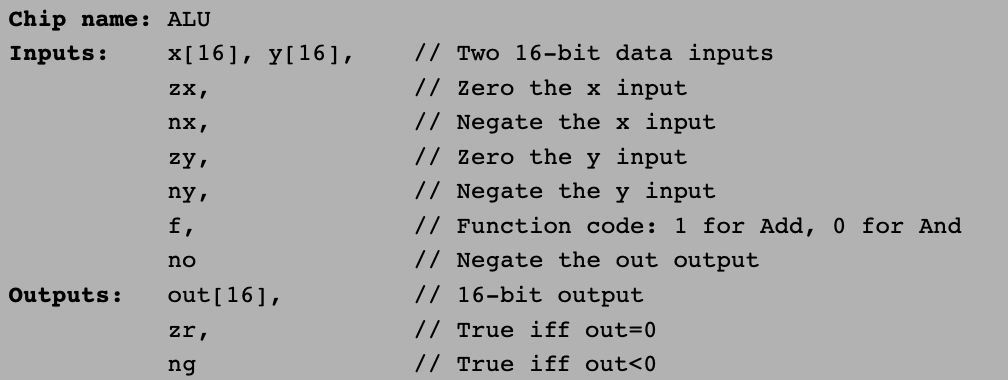
\includegraphics[scale=0.8]{pictures/alu-inp-oup.png}
	\caption{The Arithmetic Logic Unit}
\end{figure}


\paragraph{Preliminaires :} A few questions before embarking on the implementation (the order of the flags is the one presented above):
\begin{itemize}
\item What is the function \(out(x,y)\) when we pass the flags as a vector \((0,1,0,1,0,1)\) ?
\item What is the function \(out(x,y)\) when we pass the flags as a vector \((0,0,1,1,0,1)\) ?
\item What is the function \(out(x,y)\) when we pass the flags as a vector \((1,1,1,1,1,1)\) ?
\item Is it possible to calculate \(x+1\) ? If yes, what should be the value of the flags?
\item Is it possible to calculate \(x-1\) ? If yes, what should be the value of the flags?
\item Is it possible to calculate \(x-y\) ? If yes, what should be the value of the flags?
\end{itemize}

%\paragraph{Output flag :} de plus, il vous est demandé de produire deux autres sorties :
%
%\begin{itemize}
%\item \(zr\), est à \(1\) si \(out(x,y) = 0\), \(0\) sinon
%\item \(ng\), est à \(1\) si \(out(x,y) < 0\), \(0\) sinon
%\end{itemize}

\paragraph{Implementation :} Now, implement the following chip:
\begin{enumerate}
\item \texttt{ALU} (15 instructions)
\end{enumerate}

\section{Memory}
\label{sec:memory}

This part is interested in logic gates whose behavior depends on time. In other words, one of the output pins can be connected to one of the input pins. This implies that in practice, this style of chip uses a clock, which will regulate the electrical signal. However, in our case, and to simplify the design of our chips, we are not going to manipulate the clock directly. Instead, we'll assume that we have a \textit{built-in} chip, like the \texttt{nand} gate given to us. This chip, called \texttt{DFF} copies its input to its output at each clock \textit{tick} (see Fig.~\ref{fig:dff}). Note that using a clock is the same as \textit{discretizing} time.

\textbf{The Hardware Simulator is a Java program that isn’t very smart about memory management.  As a result, you should use the built-in versions of lower level RAM devices when constructing larger RAM devices (after you understand how to make the lower-level devices). Otherwise, the Hardware Simulator will recursively generate a ton of memory-resident software objects, each representing one of the parts that make up a typical RAM device. This may cause the simulator program to run slowly or to run out of memory. Hence, the folders have been divided into "a" and "b" to avoid this problem.}


\begin{figure}[h!]
  \centering
  \label{fig:dff}
  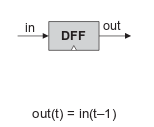
\includegraphics{pictures/dff.png}
  \caption{DFF}
\end{figure}

For this section, program the chips in the following order:

\begin{enumerate}
\item \texttt{Bit} (2 instructions)
\item \texttt{Register} (16 instructions) 
\item \texttt{PC} (5 instructions) 
\item \texttt{RAM8} (10 instructions)
\item \texttt{RAM64} (10 instructions) 
\item \texttt{RAM512} (10 instructions) 
\item \texttt{RAM4K} (10 instructions)  
\item \texttt{RAM16K} (6 instructions) 
\end{enumerate}


%\section{Computer}
%\label{sec:computer}
%
%In this part, we will reuse the RAM built in the previous part as well as our ALU to build a \textit{real} computer. Our computer will use two external peripherals: a keyboard and a screen (which are built-in), and whose specification is given to you respectively in Fig.~\ref{fig:keyboard} and Fig.~\ref{fig:screen}. Note that the Hardware Simulator manages the inputs /outputs for you. In our case, we will not take care of the entries. In the Hardware Simulator, under the option \textbf{View} you can select \textbf{Screen} to see what some tests produce (like \texttt{ComputerRect-external.tst}). Implement the chips in the following order:
%
%\begin{enumerate}
%\item \texttt{Memory} (7 instructions) 
%\item \texttt{CPU} (20 instructions) 
%\item \texttt{Computer} (3 instructions)
%\end{enumerate}
%
%In order to help you, you will find in Fig.~\ref{fig:cpu}, a diagram which summarizes the internal behavior of the CPU, and also the computer.
%
%\begin{figure}[h!]
%	\centering
%	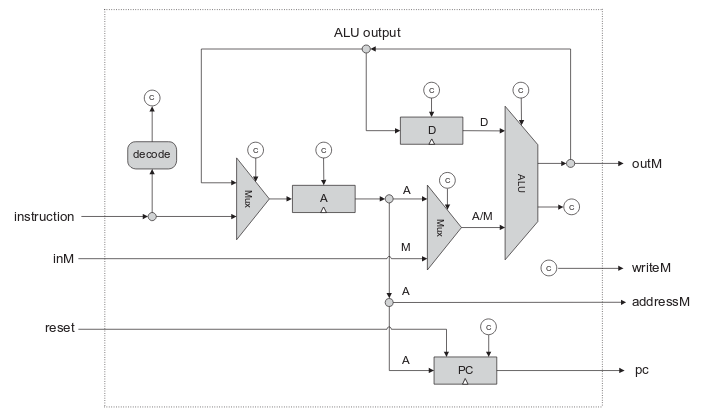
\includegraphics[scale=0.5]{pictures/cpu.png}
%	\caption{CPU}
%	\label{fig:cpu}
%\end{figure}
%
%\begin{figure}[h!]
%	\centering
%	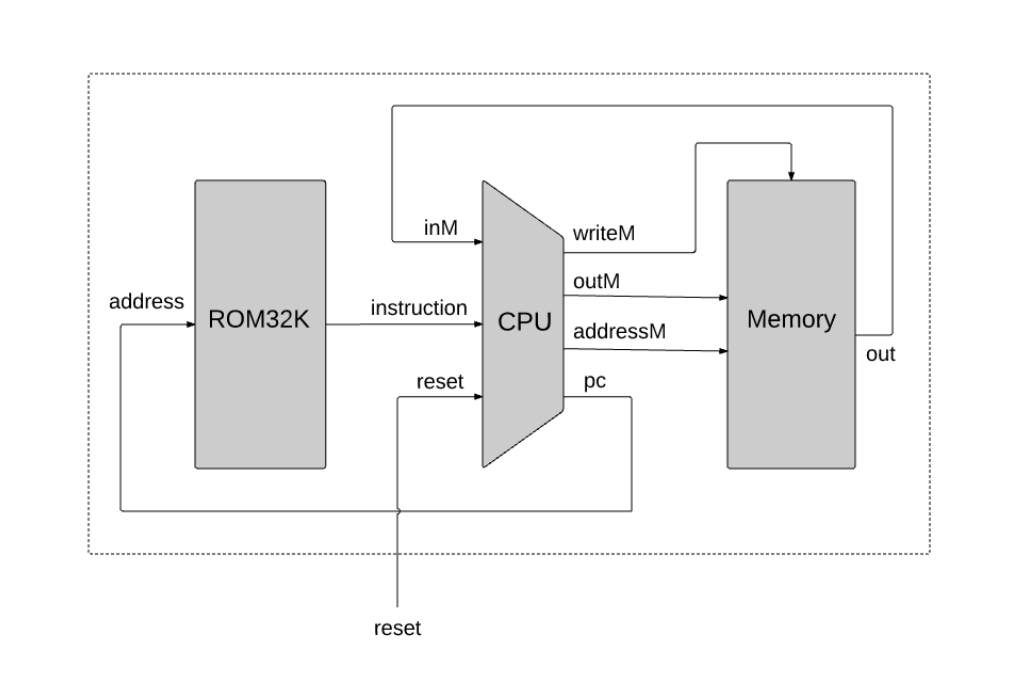
\includegraphics[scale=0.5]{pictures/cmp.png}
%	\caption{Computer}
%	\label{fig:comp}
%\end{figure}
%
%
%\begin{figure}[]
%  \centering
%\begin{verbatim}
%Chip Name:
%Keyboard    // Memory map of the physical keyboard.
%            // Outputs the code of the currently
%            // pressed key.
%Output:
%out[16]     // The ASCII code of the pressed key, or
%            // one of the special codes
%Function:
%Outputs the code of the key presently pressed on the
%physical keyboard.
%Comment:
%This chip is continuously being refreshed from a
%physical keyboard unit (simulators must simulate this
%service).
%\end{verbatim}
%
%  \caption{Keyboard}
%  \label{fig:keyboard}
%\end{figure}
%\begin{figure}[]
%  \centering
%\begin{verbatim}
%Chip Name:
%Screen       // Memory map of the physical screen
%Inputs:
%in[16],      // What to write
%load,        // Write-enable bit
%address[13]  // Where to write
%Output:
%out[16]      // Screen value at the given address
%Function:
%Functions exactly like a 16-bit 8K RAM:
%1. out(t)=Screen[address(t)](t)
%2. If load(t-1) then Screen[address(t-1)](t)=in(t-1)
%(t is the current time unit, or cycle)
%Comment:
%Has the side effect of continuously refreshing a 256
%by 512 black-and-white screen (simulators must
%simulate this device). Each row in the physical
%screen is represented by 32 consecutive 16-bit words,
%starting at the top left corner of the screen. Thus
%the pixel at row r from the top and column c from the
%left (0<=r<=255, 0<=c<=511) reflects the c%16 bit
%(counting from LSB to MSB) of the word found at
%Screen[r*32+c/16].
%\end{verbatim}
%
%  \caption{Screen}
%  \label{fig:screen}
%\end{figure}
%
% In addition, in our architecture, we must load our program in memory which will be different from the \texttt{RAM}. Here it will be the \texttt{ROM}. For that, we will also use a \textit{built-in} chip which will simulate this component see Fig.~\ref{fig:rom}.
% \begin{figure}[]
% 	\centering
% 	\begin{verbatim}
% 		Chip Name:
% 		ROM32K            // 16-bit read-only 32K memory
% 		Input:
% 		address[15]       // Address in the ROM
% 		Output:
% 		out[16]           // Value of ROM[address]
% 		Function:
% 		out=ROM[address]  // 16-bit assignment
% 		Comment:
% 		The ROM is preloaded with a machine language program.
% 		Hardware implementations can treat the ROM as a
% 		built-in chip. Software simulators must supply a
% 		mechanism for loading a program into the ROM.
% 	\end{verbatim}
% 	\caption{ROM}
% 	\label{fig:rom}
% \end{figure}
%\pagebreak
%
%We now look more closely at the specifications of the machine language. Our objective is to come up with a logic gate architecture capable of (i) executing a given instruction, and (ii) determining which
%instruction should be fetched and executed next. In order to do so, the proposed CPU
%implementation includes an ALU chip capable of computing arithmetic/logical functions, a set of
%registers, a program counter, and some additional gates designed to help decode, execute, and
%fetch instructions. Since all these building blocks were already built in previous chapters, the
%key question that we face now is how to arrange and connect them in a way that effects the
%desired CPU operation. 
%
%The architecture shown in Fig.~\ref{fig:cpu} is used to perform three classical CPU tasks: decoding
%the current instruction, executing the current instruction, and deciding which instruction to fetch
%and execute next. We now turn to describe these three tasks.
%
%\subsection*{Instruction decoding}
%The 16-bit value of the CPU’s instruction input represents either an \texttt{A-instruction} or a \texttt{C-instruction}. In order to figure out the semantics of this instruction, we can parse, or unpack it,
%into the following fields: \texttt{ixxaccccccdddjjj}. The \texttt{i}-bit (also known as opcode) codes the
%instruction type, which is either 0 for an \texttt{A-instruction} or 1 for a \texttt{C-instruction}. In case of an \texttt{A-instruction}, the entire instruction represent the 16-bit value of the constant that should be loaded
%into the A register. In case of a \texttt{C-instruction}, the \texttt{a}- and \texttt{c}-bits code the comp part of the instruction, while the \texttt{d}- and \texttt{j}-bits code the \texttt{dest} and \texttt{jump} parts of the instruction, respectively
%(the \texttt{x}-bits are not used, and can be ignored). 
%
%\subsection*{Instruction execution}
%The decoded fields of the instruction (\texttt{i}-, \texttt{a}-, \texttt{c}-, \texttt{d}-, and \texttt{j}-bits) are routed simultaneously to various parts of the CPU architecture, where they cause different chip-parts to do what they are supposed to do in order to execute either the A- or the C-instruction, as mandated by the
%machine language specification. In the case of a C-instruction, the single \texttt{a}-bit determines
%whether the ALU will operate on the A register input or on the M input, and the six \texttt{c}-bits
%determine which function the ALU will compute. The three \texttt{d}-bits are used to determine which
%registers should “accept” the ALU resulting output, and the three \texttt{j}-bits are used to for branching
%control, which can be seen in the following figures.
%
%\begin{figure}[h!]
%	\centering
%	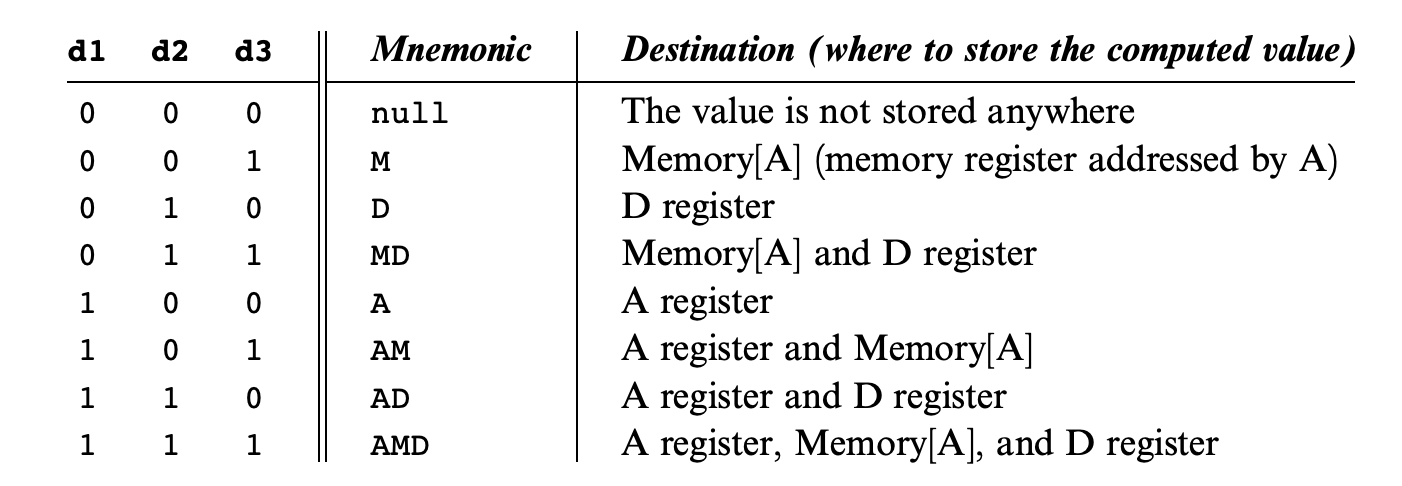
\includegraphics[scale=0.5]{pictures/dst.png}
%	\caption{The dest field of the C-instruction}
%	\label{fig:dst}
%\end{figure}
%
%\begin{figure}[h!]
%	\centering
%	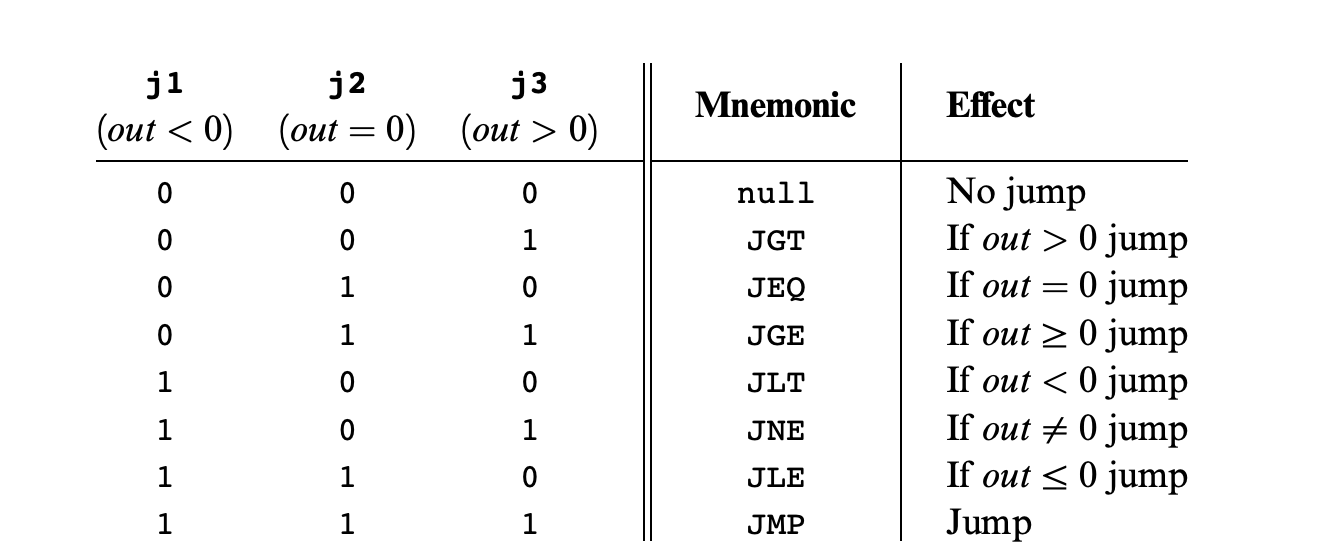
\includegraphics[scale=0.5]{pictures/jmp.png}
%	\caption{The jump field of the C-instruction. Out refers to the ALU output (resulting from
%		the instruction’s comp part), and jump implies ‘‘continue execution with the instruction
%		addressed by the A register.’’}
%	\label{fig:jmp}
%\end{figure}

\end{document}
